\documentclass[12pt]{article}
\usepackage{fancyhdr}
\usepackage{amsmath,amsfonts,enumerate}
\usepackage{color,graphicx}
\usepackage{tikz}
\usepackage{pgfplots}
\usepackage{listings}
\usepackage{algorithm}
\usepackage{algorithmic}
\usetikzlibrary{arrows,positioning,shapes,calc,matrix}
\pagestyle{fancy}
%%%%%%%%%%%%%%%%%%%%%%%%%%%%%%%%%%%%%%%%%%%%%%%%%
% Course customization based on Professor's teaching
%%%%%%%%%%%%%%%%%%%%%%%%%%%%%%%%%%%%%%%%%%%%%%%%%
\newcommand{\masunitnumber}{CENG 403}
\newcommand{\examdate}{January 2025}
\newcommand{\academicyear}{2024-2025}
\newcommand{\semester}{I}
\newcommand{\coursename}{Deep Learning - CNN Visualization \& Classic Architectures}
\newcommand{\numberofhours}{3}
%%%%%%%%%%%%%%%%%%%%%%%%%%%%%%%%%%%%%%%%%%%%%%%%%
% CUSTOM SPACING COMMANDS FOR ANSWER SPACES
%%%%%%%%%%%%%%%%%%%%%%%%%%%%%%%%%%%%%%%%%%%%%%%%%
\newcommand{\answerspace}[1]{\vspace{#1}}
\newcommand{\questionspace}{\vspace{3cm}}        
\newcommand{\subquestionspace}{\vspace{2.5cm}}   
\newcommand{\shortanswer}{\vspace{2cm}}          
\newcommand{\mediumanswer}{\vspace{3cm}}         
\newcommand{\longanswer}{\vspace{4cm}}           
\newcommand{\journalspace}{\vspace{4.5cm}}       
\newcommand{\codespace}{\vspace{5cm}}            
%%%%%%%%%%%%%%%%%%%%%%%%%%%%%%%%%%%%%%%%%%%%%%%%%
% Header setup
%%%%%%%%%%%%%%%%%%%%%%%%%%%%%%%%%%%%%%%%%%%%%%%%%
\lhead{}
\rhead{}
\chead{{\bf MIDDLE EAST TECHNICAL UNIVERSITY}}
\lfoot{}
\rfoot{}
\cfoot{}
\begin{document}
\setlength{\headsep}{5truemm}
\setlength{\headheight}{14.5truemm}
\setlength{\voffset}{-0.45truein}
\renewcommand{\headrulewidth}{0.0pt}
\begin{center}
SEMESTER \semester\ EXAMINATION \academicyear
\end{center}
\begin{center}
{\bf \masunitnumber\ -- \coursename}
\end{center}
\vspace{20truemm}
\noindent \examdate\hspace{45truemm} TIME ALLOWED: \numberofhours\ HOURS
\vspace{19truemm}
\hrule
\vspace{19truemm}
\noindent\underline{INSTRUCTIONS TO CANDIDATES}
\vspace{8truemm}
%%%%%%%%%%%%%%%%%%%%%%%%%%%%%%%%%%%%%%%%%%%%%%%%%%%%%%
% Instructions based on professor's emphasis
%%%%%%%%%%%%%%%%%%%%%%%%%%%%%%%%%%%%%%%%%%%%%%%%%%%%%%
\begin{enumerate}
\item This examination paper contains {\bf SIX (6)} questions and comprises 
{\bf EIGHT (8)} printed pages.
\item Answer all questions. 
The marks for each question are indicated at the beginning of each question.
\item Answer each question beginning on a {\bf FRESH} page of the answer book.
\item This {\bf IS NOT an OPEN BOOK} exam.
\item Show clear reasoning for your answers, especially intuitive explanations.
\item For architectural diagrams, draw clear components and explain design choices.
\item Connect concepts to examples discussed in lectures where relevant.
\item Explain the practical implications of design decisions.
\end{enumerate}
%%%%%%%%%%%%%%%%%%%%%%%%%%%%%%%%%%%%%%%%%%%%%%%%%
% New page for questions
%%%%%%%%%%%%%%%%%%%%%%%%%%%%%%%%%%%%%%%%%%%%%%%%%
\newpage
\lhead{}
\rhead{\masunitnumber}
\chead{}
\lfoot{}
\cfoot{\thepage}
\rfoot{}
\setlength{\footskip}{45pt}
%%%%%%%%%%%%%%%%%%%%%%%%%%%%%%%%%%%%%%%%%%%%%%%%%%
% EXAM QUESTIONS BASED ON PROFESSOR'S TEACHING
%%%%%%%%%%%%%%%%%%%%%%%%%%%%%%%%%%%%%%%%%%%%%%%%%%

\paragraph{Question 1. Class Activation Maps and Global Average Pooling}{\hfill (25 marks)}\\
Based on the professor's explanation: "Each channel actually specializes in capturing one part or maybe the whole part of an object... it functions as a confidence map over pixels."

\begin{enumerate}[(a)]
    \item The professor explained that global average pooling forces each channel to specialize. Explain how class activation maps exploit this property to visualize what the network is "paying attention to." Include the mathematical process of weighting channels. \hfill (10 marks)
    
    \mediumanswer
    
    \item Compare class activation maps with Grad-CAM as described by the professor. Explain why Grad-CAM replaces learned weights with "summation of gradients with respect to the channel" and how this makes the visualization "input dependent." \hfill (10 marks)
    
    \mediumanswer
    
    \item The professor mentioned that "if you do this with a CNN that has fully connected layers you are not going to get such activation maps." Explain why global average pooling is essential for class activation maps and why fully connected layers prevent this visualization. \hfill (5 marks)
    
    \shortanswer
\end{enumerate}

\newpage
\paragraph{Question 2. Feature Inversion and Network Understanding}{\hfill (22 marks)}\\
The professor discussed: "Given the feature vector for X we can try to generate an image whose feature vector is similar to that image."

\begin{enumerate}[(a)]
    \item Formulate the feature inversion optimization problem as the professor described. Explain why this is useful for understanding "what the CNN is doing" and "what level of detail it has kept and captured at different layers." \hfill (8 marks)
    
    \mediumanswer
    
    \item The professor showed reconstructions from different CNN layers. Explain his observation: "In the earlier layers information is redundant and we are able to capture the low-level details... when you go up in the network low-level details are lost." \hfill (8 marks)
    
    \mediumanswer
    
    \item The professor mentioned regularization terms to make generated images "visually pleasing." List and explain the regularization terms he discussed for controlling "smoothness" and ensuring "neighboring pixels have similar intensities." \hfill (6 marks)
    
    \shortanswer
\end{enumerate}

\newpage
\paragraph{Question 3. Adversarial Attacks}{\hfill (23 marks)}\\
Based on the professor's explanation: "We can generate a noise image that's called R with a very small magnitude such that when you add this noise image to the original image human eye is not able to visually distinguish this from the original."

\begin{enumerate}[(a)]
    \item Formulate the adversarial attack optimization problem as described by the professor. Distinguish between "targeted attack" (where "we have a target class in mind") and "untargeted attack" (where "as long as the correct class is not predicted it doesn't matter"). \hfill (8 marks)
    
    \mediumanswer
    
    \item Explain the difference between "white box approach" and "black box approach" for generating adversarial attacks. Describe the professor's explanation of using a "proxy network that mimics the predictions of the blackbox model." \hfill (8 marks)
    
    \mediumanswer
    
    \item The professor discussed serious implications: autonomous cars could "misdetect a traffic sign" or "miss a crossing." Explain why adversarial robustness is challenging, including the professor's point about decision boundaries and the "trade-off between robustness and accuracy." \hfill (7 marks)
    
    \mediumanswer
\end{enumerate}

\newpage
\paragraph{Question 4. AlexNet Architecture and Design}{\hfill (25 marks)}\\
The professor described AlexNet as "the 2012 ImageNet winner" with "60 million parameters" that had to be "split into two branches" because "they were not able to fit the whole network into a single GPU."

\begin{enumerate}[(a)]
    \item Analyze the AlexNet architecture as described by the professor. Explain why they used "a stride of four" in the first layer and why this "huge reduction in dimensionality" worked in early layers but "would lose performance if tried in the top of the network." \hfill (10 marks)
    
    \mediumanswer
    
    \item The professor found it "striking" that AlexNet filters showed specialization: one GPU learned "more or less color insensitive" filters while the other learned "more color selective filters." Explain this phenomenon and what it suggests about "group convolution." \hfill (8 marks)
    
    \mediumanswer
    
    \item List the key techniques AlexNet used to "mitigate overfitting" as mentioned by the professor, including their approach to "manually" decaying learning rate when "the loss was not improving." \hfill (7 marks)
    
    \shortanswer
\end{enumerate}

\newpage
\paragraph{Question 5. GoogleNet and Inception Modules}{\hfill (30 marks)}\\
The professor explained GoogleNet's contributions: reducing parameters "from 60 million in AlexNet to 4 million" while achieving better performance.

\begin{enumerate}[(a)]
    \item Explain the motivation for inception modules as described by the professor: "information can exist at multiple scales" and "if you use a fixed receptive field size at a layer actually you are restricting the type of information you can extract to only a fixed scale." \hfill (8 marks)
    
    \mediumanswer
    
    \item The professor described the "scalability problem" with naive inception modules: "the number of channels explodes." Draw the improved inception module and explain how "one by one convolution" solves this by ensuring "if the input layer has C channels the output layer after concatenation has C many channels as well." \hfill (12 marks)
    
    \begin{center}
    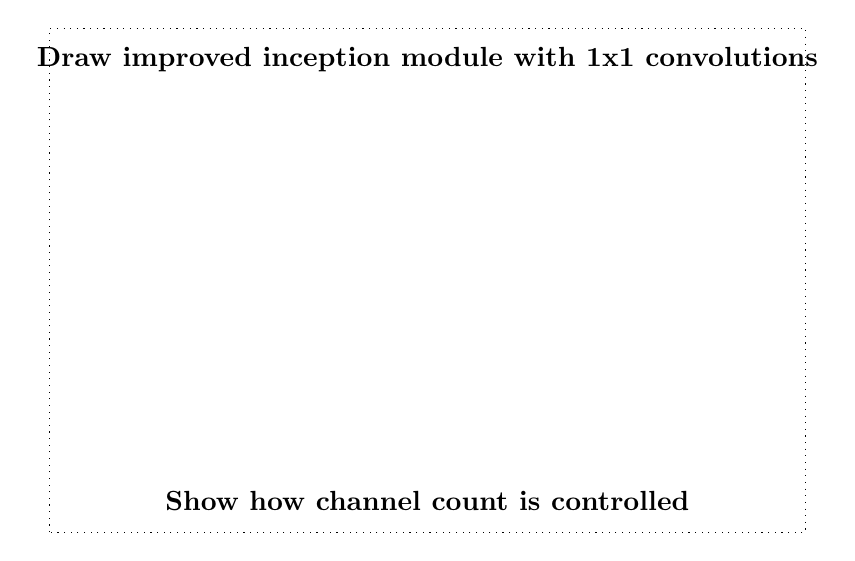
\begin{tikzpicture}[scale=0.8]
        % Space for inception module drawing
        \draw[dotted] (0,0) rectangle (12,8);
        \node at (6,7.5) {\textbf{Draw improved inception module with 1x1 convolutions}};
        \node at (6,0.5) {\textbf{Show how channel count is controlled}};
    \end{tikzpicture}
    \end{center}
    
    \shortanswer
    
    \item Explain GoogleNet's second contribution: "adding fully connected layers into the intermediate layers of the network." Discuss both benefits (gradient flow, multi-scale recognition) and drawbacks (reproducibility issues, loss of generalization) as mentioned by the professor. \hfill (10 marks)
    
    \mediumanswer
\end{enumerate}

\newpage
\paragraph{Question 6. ResNet and Skip Connections}{\hfill (25 marks)}\\
The professor explained the key insight: "After a certain number of layers performance doesn't improve... it actually becomes even worse" and ResNet's solution using skip connections.

\begin{enumerate}[(a)]
    \item Analyze the professor's explanation of why deeper networks perform worse: "when you multiply all those gradients through all of these layers you don't get useful gradients to the earlier parts of the network." Explain why this isn't simply overfitting. \hfill (8 marks)
    
    \mediumanswer
    
    \item Draw a ResNet block and explain the professor's description: "in forward pass we have a function of the input as well as the identity being propagated" and "in backward pass gradient will flow through two paths." \hfill (10 marks)
    
    \begin{center}
    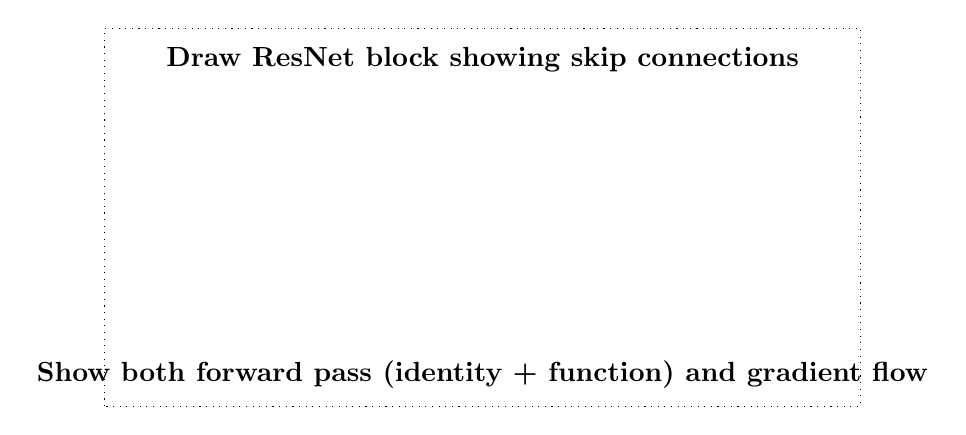
\begin{tikzpicture}[scale=0.8]
        % Space for ResNet block drawing
        \draw[dotted] (0,0) rectangle (12,6);
        \node at (6,5.5) {\textbf{Draw ResNet block showing skip connections}};
        \node at (6,0.5) {\textbf{Show both forward pass (identity + function) and gradient flow}};
    \end{tikzpicture}
    \end{center}
    
    \shortanswer
    
    \item The professor mentioned two interpretations of why ResNet works: the "smoother loss function" hypothesis and viewing ResNet as "an ensemble of multiple sub networks." Explain both interpretations and discuss why "there is no theorem showing this." \hfill (7 marks)
    
    \mediumanswer
\end{enumerate}

\vfill
\begin{center}{\bf END OF PAPER}\end{center>
\end{document}